\documentclass[a4paper,10pt]{article}
\usepackage[utf8]{inputenc}
\usepackage[T1]{fontenc}
\usepackage[french]{babel}
\usepackage{amsmath}
\usepackage{hyperref}
\usepackage{amsfonts}
\usepackage{graphicx}

\begin{document}
\title{Rapport TER}
\author{Raphaël Muller,Billel Guerfa}
\maketitle

\part{Introduction}
\par
L'apprentissage machine (Machine Learning) est une branche de l'intelligence artificielle permettant à un système d'apprendre et d'améliorer ses performances par l'expérience et une mesure de ces dernières, et donc sans être explicitement programmé, récemment et notamment grâce aux avancées en terme de hardware, cette branche de l'IA a révolutionnée le domaine et a donnée naissance à bon nombre d'applications (Systèmes de reconnaissances d'images, détection d'anomalies, voitures autonomes, bots joueurs...) et ainsi résolu beaucoup de problèmes qui sont difficiles à approcher en utilisant les techniques algorithmiques classiques.
\par
Il y a trois types d'approches pour résoudre un problème en apprentissage automatique :
\begin{itemize}
\item  \textbf{L'apprentissage supervisé:} cette approche est intéressante dés qu'on a plusieurs instances de notre problème (représentant un large échantillon représentatif) ainsi que les solutions correctes pour chaque instance, qu'on appelle labels, ici on vise à déduire un modèle représentant notre problème i.e, une fonction qui prend en paramètres les données observables du problème et qui nous en donne la solution, cette fonction aura des paramètres internes qui seront "appris" ou optimisés par notre algorithme afin de construire le meilleur modèle possible Ex (Classifications d'images).
    
\item \textbf{L'apprentissage non-supervisé:} dans ce cas, on ne sait pas donner a notre algorithme les solutions correctes pour les instances de notre problème, mais on lui demandera de déduire une structure et des informations à partir de ces instances (Clustering , Word Embeddings afin de déduire le lien sémantique entre les mots dans une langue).

\item \textbf{L'apprentissage par renforcement:} cette dernière branche est considérée comme la plus prometteuse et la plus active en recherche car c'est le premier pas vers une intelligence artificielle générale, c'est pour cette raison qu'elle est très utilisée dans des environnements complexes comme pour les jeux ainsi que les voitures autonomes, elle se base sur le principe qu'on a un agent qui observe un environnement et qui choisit de soumettre des actions à ce dernier, l'environnement ensuite lui envoie une nouvelle observation, ainsi qu'une récompense ou une pénalité, l'agent optimisera ses actions en fonction des récompenses qu'il reçoit et aura donc tendance à privilégier les états ou il peut avoir le plus de récompenses possibles.
\end{itemize}
     

\par
On entend aussi beaucoup parler du Deep Learning, contrairement aux approches citées précédemment, le deep learning est plus un moyen ou une structure adaptée pour des calculs intensifs (les réseaux de neurones), qu'une approche. On peut utiliser le deep learning en apprentissage supervisé, non supervisé, ainsi qu'en apprentissage par renforcement (Deep reinforcement learning) il est également trés utilisé dans le domaine du big data (partie analytique) en raison du volume massif de données à analyser.


\par
Dans le cadre de notre projet, on explore l'approche de l'apprentissage par renforcement et ses différents algorithmes afin de créer un agent capable de jouer et d'améliorer ses performances sur le jeu de plateau Ignis, on présentera donc une modélisation d'un processus de décision de Markov, ainsi que sa résolution par une méthode d'apprentissage par renforcement.


\part{Théorie}
\section{Processus de décision de Markov}
\subsection{Processus de Markov}
Le processus de décision de Markov décrit formellement un environnement pour l' apprentissage par renforcement. Cet environnement est totalement observable et dénombrable.
Les chaines vérifient toutes la propriété de Markov. Un état $S_t$ vérifie les propriété de Markov si et seulement si:
\[\mathbb{P}[S_{t+1}|S_t]=\mathbb{P}[S_{t+1}|S_1,....,S_t]\]
Cela signifie que l'état $S_t$ a  une propriété d'absence de mémoire, c'est a dire que l'état actuel contient toutes les informations importantes des états précédents . Cela permet donc d'ignorer l'historique des états précédents.
\par
Pour un état de Markov s et un état suivant s', l'état de transition est défini par : \[P_{ss'}=\mathbb{P}[S_{t+1}=s'|S_t=s]\]
Une matrice de transition P défini les probabilités de transitions d'un état s vers tous ses successeurs s' \[P = s
\begin{tabular}{c}
 s'\\
$$$\begin{bmatrix}
P_{11} & P_{12} & P_{13} \\
P_{21} & P_{22} & P_{23} \\
P_{31} & P_{32} & P_{33}
\end{bmatrix}$$$\\
\\
\end{tabular}\]
Ici $P_{12}$ est la probabilité d'aller vers l'état 2 quand on se trouve dans l'état 1. De ce fait la somme de chaque ligne de la matrice vaut 1.\par
Une chaine de Markov est une suite de variables aléatoires $S_1,S_2$... tel avec les propriétés de Markov. Un processus de Markov(ou chaine de Markov) est un couple (S,P)
\begin{itemize}
\item[S] est un ensemble d'états supposé fini
\item[z] est une matrice de transitions 
\end{itemize}
\subsection{Processus de récompense de Markov}
Un Processus de récompense de Markov est une chaine de Markov avec des valeurs, défini par(S,P,R,$\gamma$) 
\begin{itemize}
\item[S] est un ensemble d'états supposé fini
\item[P] est une matrice de transitions 
\item[R] est la fonction de récompense $R_s = \mathbb{E}[R_{t+1}|S_t =s]$
\item[$\gamma$] est un facteur de réduction, $\gamma \in [0,1]$
\end{itemize}
\vspace{12pt}
Le résultat $G_t$ est le total des récompenses réduites depuis l'itération t.C'est une variable aléatoire.
\[G_t = R_{t+1}+\gamma R_{t+2}+...= \sum_{k=0}^{\infty}\gamma^k R_{t+k+1}\]
$\gamma$ sert a réduire la valeur de $R_k$ plus k est grand puisque on met $\gamma$ a la puissance k. Cela va mener, si  $\gamma$ est proche de 0, à une évaluation au court terme; et à une évaluation au long terme si  $\gamma$ est proche de 1. La réduction permet d'éviter les cycles dans les chaines de Markov  et permet de valoriser les récompenses au court terme 
La \textit{value function} $v(s)$ d'un processus de récompense de Markov est un fonction qui retourne la valeur au long terme en partant d'un état s. Cela représente l'espérance du retour de $G_t$.
\[v(s)=\mathbb{E}[G_t|S_t=s]\]
équation que nous pouvons réduire:
\[
\begin{aligned}
v(s)&=\mathbb{E}[G_t|S_t=s]\\
&=\mathbb{E}[R_{t+1}+\gamma R_{t+2}+\gamma^2R_{t+3}+...|S_t=s]\\
&=\mathbb{E}[R_{t+1}+\gamma(R_{t+2}+\gamma R_{t+3}+...)|S_t=s]\\
&=\mathbb{E}[R_{t+1}+\gamma G_t+1 |S_t=s]\\
&=\mathbb{E}[R_{t+1}+\gamma v(S_{t+1}) |S_t=s]
\end{aligned}
\]
La value function peut donc être divisé en deux parties, la récompense immédiate et la value function du successeur. Nous obtenons une équation de Bellman.
C'est une équation décrivant un problème de programmation dynamique c'est a dire que la valeur obtenue dépend du résultat de cette même fonction de façon récursive qui prend en compte l'état initial.
\\
cette équation peut être résumée en :
\[v(s)=R_s + \gamma \sum_{s'\in S} P_{ss'}v(s')\]
ce qui signifie que la \textit{value function} est égale a la récompense de l'état courant, plus la somme des values function des états suivants multiplié par leur probabilité d'être choisis, cette somme étant réduite par le facteur $\gamma$.\par
On peut résumer cette équation de Bellman en utilisant des vecteurs et matrices.
\[v=R+\gamma Pv\]
\begin{itemize}
\item[v] est le vecteur des value function
\item[R] est le vecteur des récompenses
\item[P] est la matrice de transition
\item[$\gamma$] est le facteur de réduction
\end{itemize}
on obtient donc une équation linéaire:
\[
\begin{aligned}
v &= R+ \gamma P v\\
(I - \gamma P)v &= R\\
v &= (I - \gamma P)^{-1} R
\end{aligned}
\]
Cette équation est en O($n^3$) pour n états ce qui n'est pas réalisable pour un nombre trop important d'états. on devra donc trouver des méthodes pour réduire cette complexité, comme la programmation dynamique,l'utilisation d'algorithmes de monte-Carlo ou l'apprentissage par différences temporelles.
\subsection{Le processus de décision de Markov}
Un processus de décision de Markov est un processus de récompense de Markov avec des décisions. Défini par (S,A,P,R,$\gamma$).
\begin{itemize}
\item[S] est un ensemble d'états supposé fini
\item[A] est un ensemble d'actions supposé fini
\item[P] est une matrice de transitions 
\item[R] est la fonction de récompense $R_s = \mathbb{E}[R_{t+1}|S_t =s]$
\item[$\gamma$] est un facteur de réduction, $\gamma \in [0,1]$
\end{itemize}
\vspace{12pt}
\subsubsection{Policies}
Une politique(\textit{policy}) $\pi$ est une distribution sur les actions A sachant les états.
\[
\pi (a|s) = \mathbb{P}[A_t = a | S_t =s]
\]

Une politique définit le comportement d'un agent. Du fait de la propriété des chaines de Markov, les \textit{policies} ne dépendent pas de l'historique ni de l'itération.
\par
la séquence d'état et de récompenses avec une \textit{policy}, est un processus de récompense de Markov noté $(S,P^{\pi},R^{\pi},\gamma)$ ou:
\par
\[
P^{\pi }_{s,s'}= \sum_{a \in A} (a|s)P^{a}_{ss'}
\]
\[
R^{\pi}_{s}=\sum_{a \in A} (a|s)R^{a}_{s}
\]


\subsubsection{La value function}
La\textit{ value function} d'un état $v_{\pi}(s)$ d'un processus de décision de markov et le résultat attendu, en partant d'un état s, et suivant une policy $\pi$

\[
v_{\pi}(s) = \mathbb{E}_{\pi}[G_t|S_t = s]
\]

La fonction d' \textit{action value} $q_{\pi}(s,a)$ est est le retour attendu en partant de l'état s, réalisant l'action a et suivant la policy $\pi$.
\[
q_{\pi}(s,a) = \mathbb{E}_{\pi}[G_t|S_t =s,A_t =a]
\]

La valeur de $v^{\pi}$ attendue par l'équation de Bellman est :
\[
v_{\pi}(s)= \sum_{a \in A} \pi (a|s)q_{\pi}(s,a)
\]

La valeur de $q^{\pi}$ attendue par l'équation de Bellman est :

\[
q_{\pi}(s,a)= R^{a}_s + \gamma \sum_{s \in S} P^{a}_{ss'}v_{\pi}(s')
\]

En retournant sous forme matriciel on a:
\[
\begin{aligned}
v_{\pi} &= R^{\pi} + \gamma P^{\pi} v*_{pi}
v_{\pi} &= (I - \gamma P^{\pi})^{-1} R^{\pi}
\end{aligned}
\]
\subsubsection{value function optimal}

la value function d'un état $v_*(s)$ est le maximum de la value function de toutes les policies:
\[
 v_*(s) = \underset{\pi}{max}* v_{\pi}(s) 
\]
\[
 q_*(s,a) =\underset{\pi}{max}*q_{\pi}(s,a) 
\]
et
\[
  v_*(s) = \underset{a}{max}*R^{a}_s \sum_{s' \in S} P^{a}_{ss'} v_* (s') 
\]
\[
q_*(s,a) = R^{a}_s + \gamma \sum_{s' \in S} P^{a}_{ss'} \underset{a'}{max}* q_*(s',a') 
\]

pour résoudre ces équations il existe quelques solutions, comme par exemple le Q-learning, la \textit{policy iteration} et la \textit{value iteration}.

\section{Organisation par programmation dynamique}
\par
La programmation dynamique est un concept servant a résoudre des problèmes d'optimisation. Elle a pour principe de diviser pour mieux régner. Elle décompose le problème en sous-problèmes plus facile a résoudre pour a la fin regrouper tous les résultats.
\par
C'est une solution générale pour les processus de décision de Markov car l'équation de Bellman décompose la  \textit{value fonction} de façon récursive et elle permet de réutiliser les résultats trouvé grâce au stockage de ces derniers.

Mais la programmation dynamique nécessite une connaissance du processus de Markov et une matrice d'une taille assez faible.
Dans notre cas, la programmation dynamique n'est pas adapté donc nous passerons rapidement sur des informations importantes.

\subsection{Policy iteration} 
\par
Étant donné une politique $\pi$ et une \textit{value iteration} $v_{\pi}$, on améliore la politique en essayant de maximiser les gains en suivant $v_{\pi}$
\[
\pi' = maximisation(v_{\pi})
\]

le but est de trouver la politique optimale, $\pi^*$

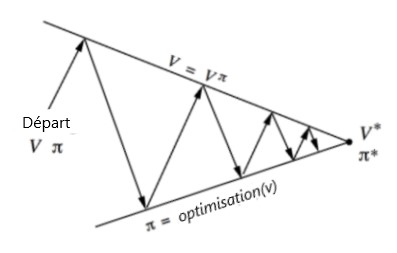
\includegraphics[scale=0.8]{image1.jpg}

\section{Estimer la valeur d'un processus de décision de Markov inconnu}

\subsection{Les méthodes de Monte-Carlo}
	
Un algorithme de Monte-Carlo est un algorithme probabiliste. TODO:  def mc

Cette méthode apprend directement depuis une expérience. elle est aussi "model-free" TODO: a traduire, c'est a dire qu'il n'a pas besoin de la connaissance de la chaine de Markov et de récompenses.
	

\end{document}